% Beamer slimmed-down version of the JRC C4 Practical Use section.
% Built from talk_v2.md content + audit applied: 12 -> 9 slides.
% Compile:  xelatex jrc_section_v2_beamer.tex  (run twice for refs)
\documentclass[aspectratio=169,11pt]{beamer}
\usepackage{fontspec}
\setsansfont{Helvetica Neue}[Scale=0.92]
\setmonofont{Menlo}[Scale=0.78]
\usepackage{xcolor}
\usepackage{graphicx}
\usepackage{tcolorbox}
\tcbuselibrary{skins,raster}
\usepackage{tikz}
\usepackage{array}

% --- palette ---
\definecolor{jrcblue}{HTML}{3B3B8C}
\definecolor{l1grey}{HTML}{7F7F7F}
\definecolor{l2amber}{HTML}{D97706}
\definecolor{l3orange}{HTML}{EA580C}
\definecolor{taskblue}{HTML}{1F77B4}
\definecolor{bggreen}{HTML}{2CA02C}
\definecolor{dontred}{HTML}{D62728}
\definecolor{cardbg}{HTML}{FAFAFA}

% beamer auto-loads hyperref; just override the colour scheme here.
\hypersetup{colorlinks=true,linkcolor=jrcblue,urlcolor=jrcblue,citecolor=jrcblue}

\usetheme{default}
\setbeamertemplate{navigation symbols}{}
\setbeamercolor{frametitle}{fg=jrcblue,bg=white}
\setbeamercolor{normal text}{fg=black,bg=white}
\setbeamerfont{frametitle}{size=\Large,series=\mdseries}
\setbeamertemplate{itemize item}{\color{jrcblue}\textbullet}
\setbeamertemplate{itemize subitem}{\color{jrcblue}\textendash}
% Footer template: slide number bottom-left, EC logo bottom-right
% (matches the JRC C4 parent deck convention).
\setbeamertemplate{footline}{%
  \leavevmode%
  \makebox[\paperwidth]{%
    \hspace{8mm}\raisebox{8pt}{\tiny\color{gray}\insertframenumber}%
    \hfill%
    \raisebox{2pt}{
\includegraphics[height=0.075\paperheight]{assets/ec_logo.png}}\hspace{6mm}%
  }%
  \vspace{2pt}%
}
\setbeamertemplate{frametitle}{%
  \vspace{6pt}\hspace{4pt}\insertframetitle\par\vspace{-4pt}%
}

% --- macros ---

% Tip card: a coloured box with TIP-label and short body.
% Usage: \tipcard{TIP 1}{Title}{Body text}
\newcommand{\tipcard}[3]{%
  \begin{tcolorbox}[
    colback=cardbg, colframe=jrcblue, boxrule=1pt, arc=3pt,
    left=8pt, right=8pt, top=4pt, bottom=4pt,
    fontupper=\small,
  ]
    {\textbf{#1}}\\[1pt]
    {\color{jrcblue}\textbf{#2}}\\[3pt]
    #3
  \end{tcolorbox}%
}

% Tight tip card: same as \tipcard but smaller padding and footnotesize body,
% used on the dense pre-experiment slide (slide 2) to fit five boxes.
\newcommand{\tipcardtight}[3]{%
  \begin{tcolorbox}[
    colback=cardbg, colframe=jrcblue, boxrule=1pt, arc=3pt,
    left=7pt, right=7pt, top=2pt, bottom=2pt,
    fontupper=\footnotesize,
  ]
    {\textbf{#1}}\\[0.5pt]
    {\color{jrcblue}\textbf{#2}}\\[2pt]
    #3
  \end{tcolorbox}%
}

% Sub-tip card: lighter chip
\newcommand{\subtipcard}[3]{%
  \begin{tcolorbox}[
    colback=cardbg, colframe=jrcblue!40, boxrule=1pt, arc=3pt,
    left=8pt, right=8pt, top=4pt, bottom=4pt,
    fontupper=\small,
  ]
    {\textbf{#1}}\\[1pt]
    {\color{jrcblue}\textbf{#2}}\\[3pt]
    #3
  \end{tcolorbox}%
}

% Level card for the experiment intro. Height set so the densest card
% (Level 3) fits without text colliding with the bottom border.
\newcommand{\levelcard}[3]{%
  \begin{tcolorbox}[
    colback=cardbg, colframe=#1, boxrule=1.2pt, arc=3pt,
    left=6pt, right=6pt, top=4pt, bottom=4pt,
    valign=top, height=3.4cm, fontupper=\small,
  ]
    \textbf{\textcolor{#1}{#2}}\\[2pt]
    \scriptsize\textcolor{gray!40!black}{#3}
  \end{tcolorbox}%
}

% Pattern boxes (TASK/BG/DO NOT) — compact variant for the L3 prompt slide
\newcommand{\patternbox}[3]{%
  \begin{tcolorbox}[
    colback=cardbg, colframe=#1, boxrule=1pt, arc=3pt,
    left=6pt, right=6pt, top=2pt, bottom=2pt,
    fontupper=\scriptsize,
  ]
    {\scriptsize\textbf{\textcolor{#1}{#2}}}\par
    \scriptsize #3
  \end{tcolorbox}%
}

\begin{document}

% ===== Slide 1 — Section divider (optional; drop if pasting into parent at slot 38) =====
{\setbeamertemplate{footline}{}
\begin{frame}[plain]
  \vfill
  \begin{center}
    {\fontsize{40pt}{44pt}\selectfont\color{jrcblue}\bfseries Practical Use Cases}\\[10pt]
    {\Large\color{gray!40!black}Seven tips, one forecasting experiment}
  \end{center}
  \vfill
  \begin{center}\small\color{gray}Speaker: Dermot O'Brien\end{center}
\end{frame}}

% ===== Slide 2 — Tips 1–5 (everything the experiment references) =====
% Layout: top row wide pair (TIPS 1, 2), bottom row narrow trio (TIPS 3, 4, 5).
% TIP 2 is the densest tip, so it gets the wider top-right cell.
% Tip-card padding is scoped tighter on this slide to fit all five boxes
% without bottom-row clipping.
\begin{frame}{Seven tips for working with AI}
  \begin{columns}[t,onlytextwidth]
    \begin{column}{0.49\textwidth}
      \tipcardtight{TIP 1}{Learn how to program, use your domain knowledge}{%
        AI multiplies what you already know. Bring expertise; AI brings throughput.}
    \end{column}
    \begin{column}{0.49\textwidth}
      \tipcardtight{TIP 2}{Be as specific as humanly possible}{%
        Most prompts don't give enough context. Paste in docs, references, \texttt{llms.txt}, screenshots.
        Or draft a rough prompt and ask AI to rewrite it \emph{``using LLM best practices.''}}
    \end{column}
  \end{columns}
  \vspace{-2pt}
  \begin{columns}[t,onlytextwidth]
    \begin{column}{0.32\textwidth}
      \tipcardtight{TIP 3}{Smaller tasks beat big ones}{%
        Break problems down. If you can't break it down, you don't understand it yet.}
    \end{column}
    \begin{column}{0.32\textwidth}
      \tipcardtight{TIP 4}{Tell the AI what you \emph{don't} want}{%
        Three-section pattern: \textbf{TASK / BACKGROUND / DO NOT}.}
    \end{column}
    \begin{column}{0.32\textwidth}
      \tipcardtight{TIP 5}{Tell AI to remember}{%
        \texttt{AGENTS.md} (context) + skills (procedures) in \texttt{.claude/}.
        Ask the agent to draft v1.}
    \end{column}
  \end{columns}
\end{frame}

% ===== Slide 4 — The experiment =====
\begin{frame}{The experiment}
  \begin{itemize}\small
    \item \textbf{Task}: forecast 168 hours of hourly German electricity load,
          2020-01-01 to 2020-01-07.
    \item \textbf{Data}: \href{https://data.open-power-system-data.org/time_series/}{Open Power System Data} (OPSD) / ENTSO-E, 2015\textendash{}2020, hourly.
    \item \textbf{Agent}: Claude Code, Opus 4.7 \textemdash{} same agent in every run.
    \item \textbf{Code, prompts, and full results}:
          \href{https://github.com/DermotOBrien-EC/LLM_coding_practical_example_JRC_LEGENT_presentation_15_05_26}%
               {github.com/DermotOBrien-EC/LLM\_coding\_practical\_example\_JRC\_LEGENT\_presentation\_15\_05\_26}
    \item \textbf{Three prompts, three workspace setups:}
  \end{itemize}
  \vspace{4pt}
  \begin{columns}[t,onlytextwidth]
    \begin{column}{0.32\textwidth}
      \levelcard{l1grey}{Level 1 \textemdash{} beginner}{%
        ``Forecast first week of January 2020 German hourly electricity load.''\\
        \textbf{10 words \textperiodcentered{} no AGENTS.md}}
    \end{column}
    \begin{column}{0.32\textwidth}
      \levelcard{l2amber}{Level 2 \textemdash{} average}{%
        Names data, horizon, libraries. Asks for plot + accuracy.\\
        \textbf{46 words \textperiodcentered{} 7-line AGENTS.md}}
    \end{column}
    \begin{column}{0.32\textwidth}
      \levelcard{l3orange}{Level 3 \textemdash{} research-grade}{%
        Structured TASK / BACKGROUND / DO NOT. 6-model bake-off, validation, intervals.\\
        \textbf{1{,}673 words \textperiodcentered{} 113-line AGENTS.md}}
    \end{column}
  \end{columns}
  \vfill
  {\tiny\color{gray!50!black}%
   OPSD time series: \href{https://data.open-power-system-data.org/time_series/}{https://data.open-power-system-data.org/time\_series/}}
\end{frame}

% ===== Slide 5 — Level 1 result =====
\begin{frame}{Level 1: what 10 words gets you}
  \small\itshape ``Forecast first week of January 2020 German hourly electricity load.''
  \vspace{4pt}
  \begin{center}
    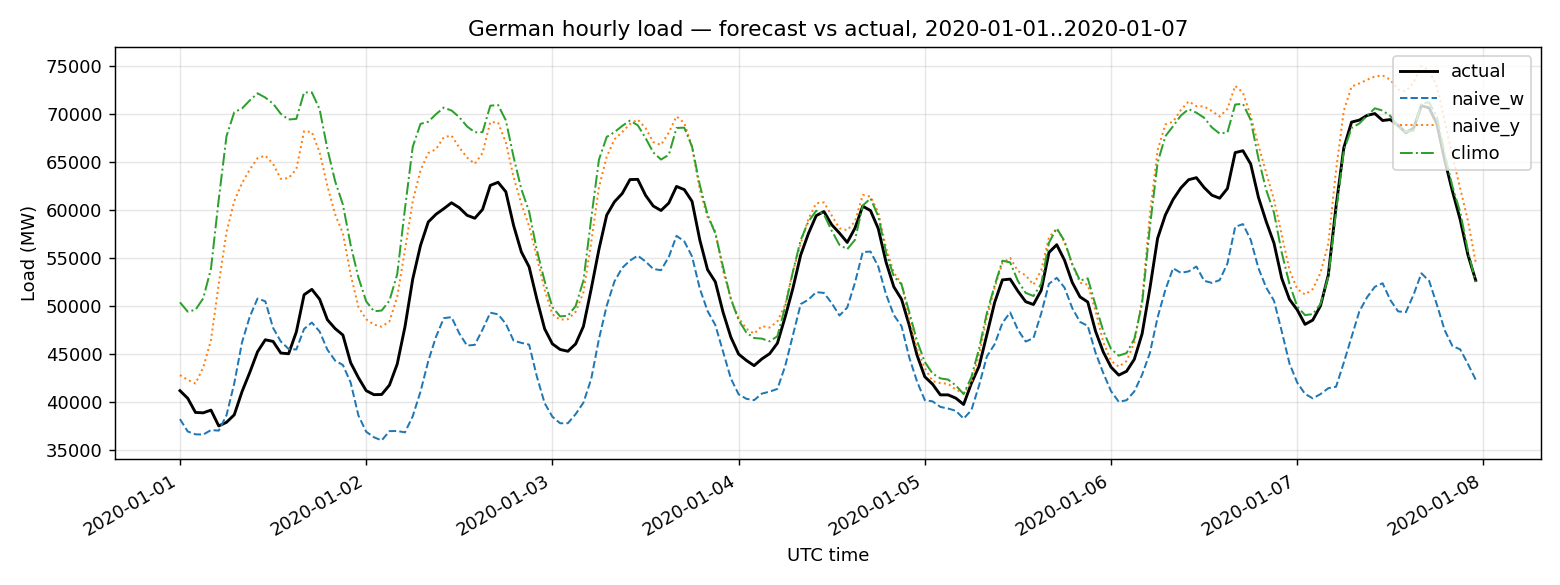
\includegraphics[height=0.58\textheight]{../runs/L1/forecast.png}
  \end{center}
  \begin{center}\small\color{gray!40!black}
    Three baselines compared; L1 picked the best of three: \textbf{seasonal-naive (lag-364d), MAPE 10.76\%}.\\
    No validation set. No prediction intervals. No methodology document.
  \end{center}
\end{frame}

% ===== Slide 6 — Level 2 result =====
\begin{frame}{Level 2: average prompt + thin workspace}
  \small\itshape ``Build me a Python script that forecasts German hourly electricity load for the first week
  of January 2020. Train on the historical data, plot it, and tell me how accurate it was.''\\
  \scriptsize\color{gray!40!black} AGENTS.md: \emph{Python project. opsd\_de\_load.csv has hourly German load. Use pandas. Plot with matplotlib.}
  \vspace{2pt}
  \begin{center}
    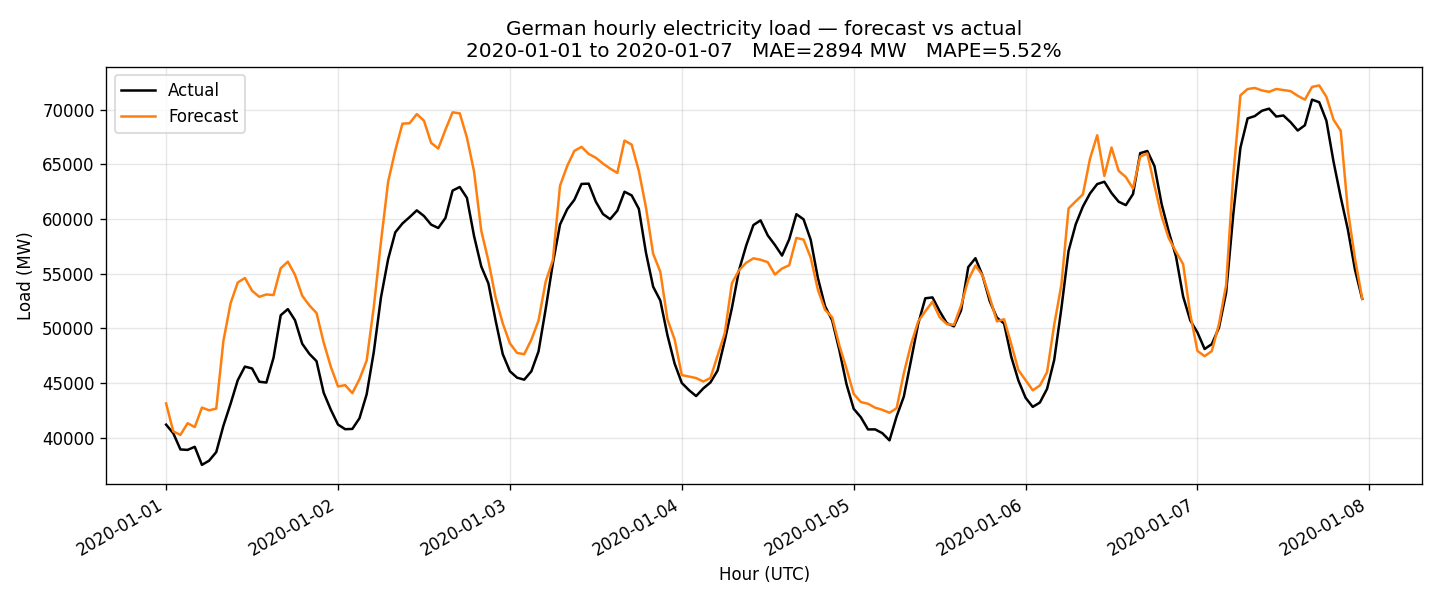
\includegraphics[height=0.50\textheight]{../runs/L2/forecast.png}
  \end{center}
  \begin{center}\small\color{gray!40!black}
    \textbf{GradientBoostingRegressor}, engineered features. \textbf{MAPE 5.52\%.}
    Still no held-out validation, no intervals, no methods document.
  \end{center}
\end{frame}

% ===== Slide 7 — Level 3 result =====
\begin{frame}{Level 3: research-grade prompt}
  \footnotesize\color{gray!40!black}
  Prompt followed the TASK / BACKGROUND / DO NOT pattern (Tip 4).
  1{,}673 words \textperiodcentered{} 113-line AGENTS.md \textperiodcentered{} 6-model bake-off with held-out validation and calibrated intervals.
  \begin{center}
    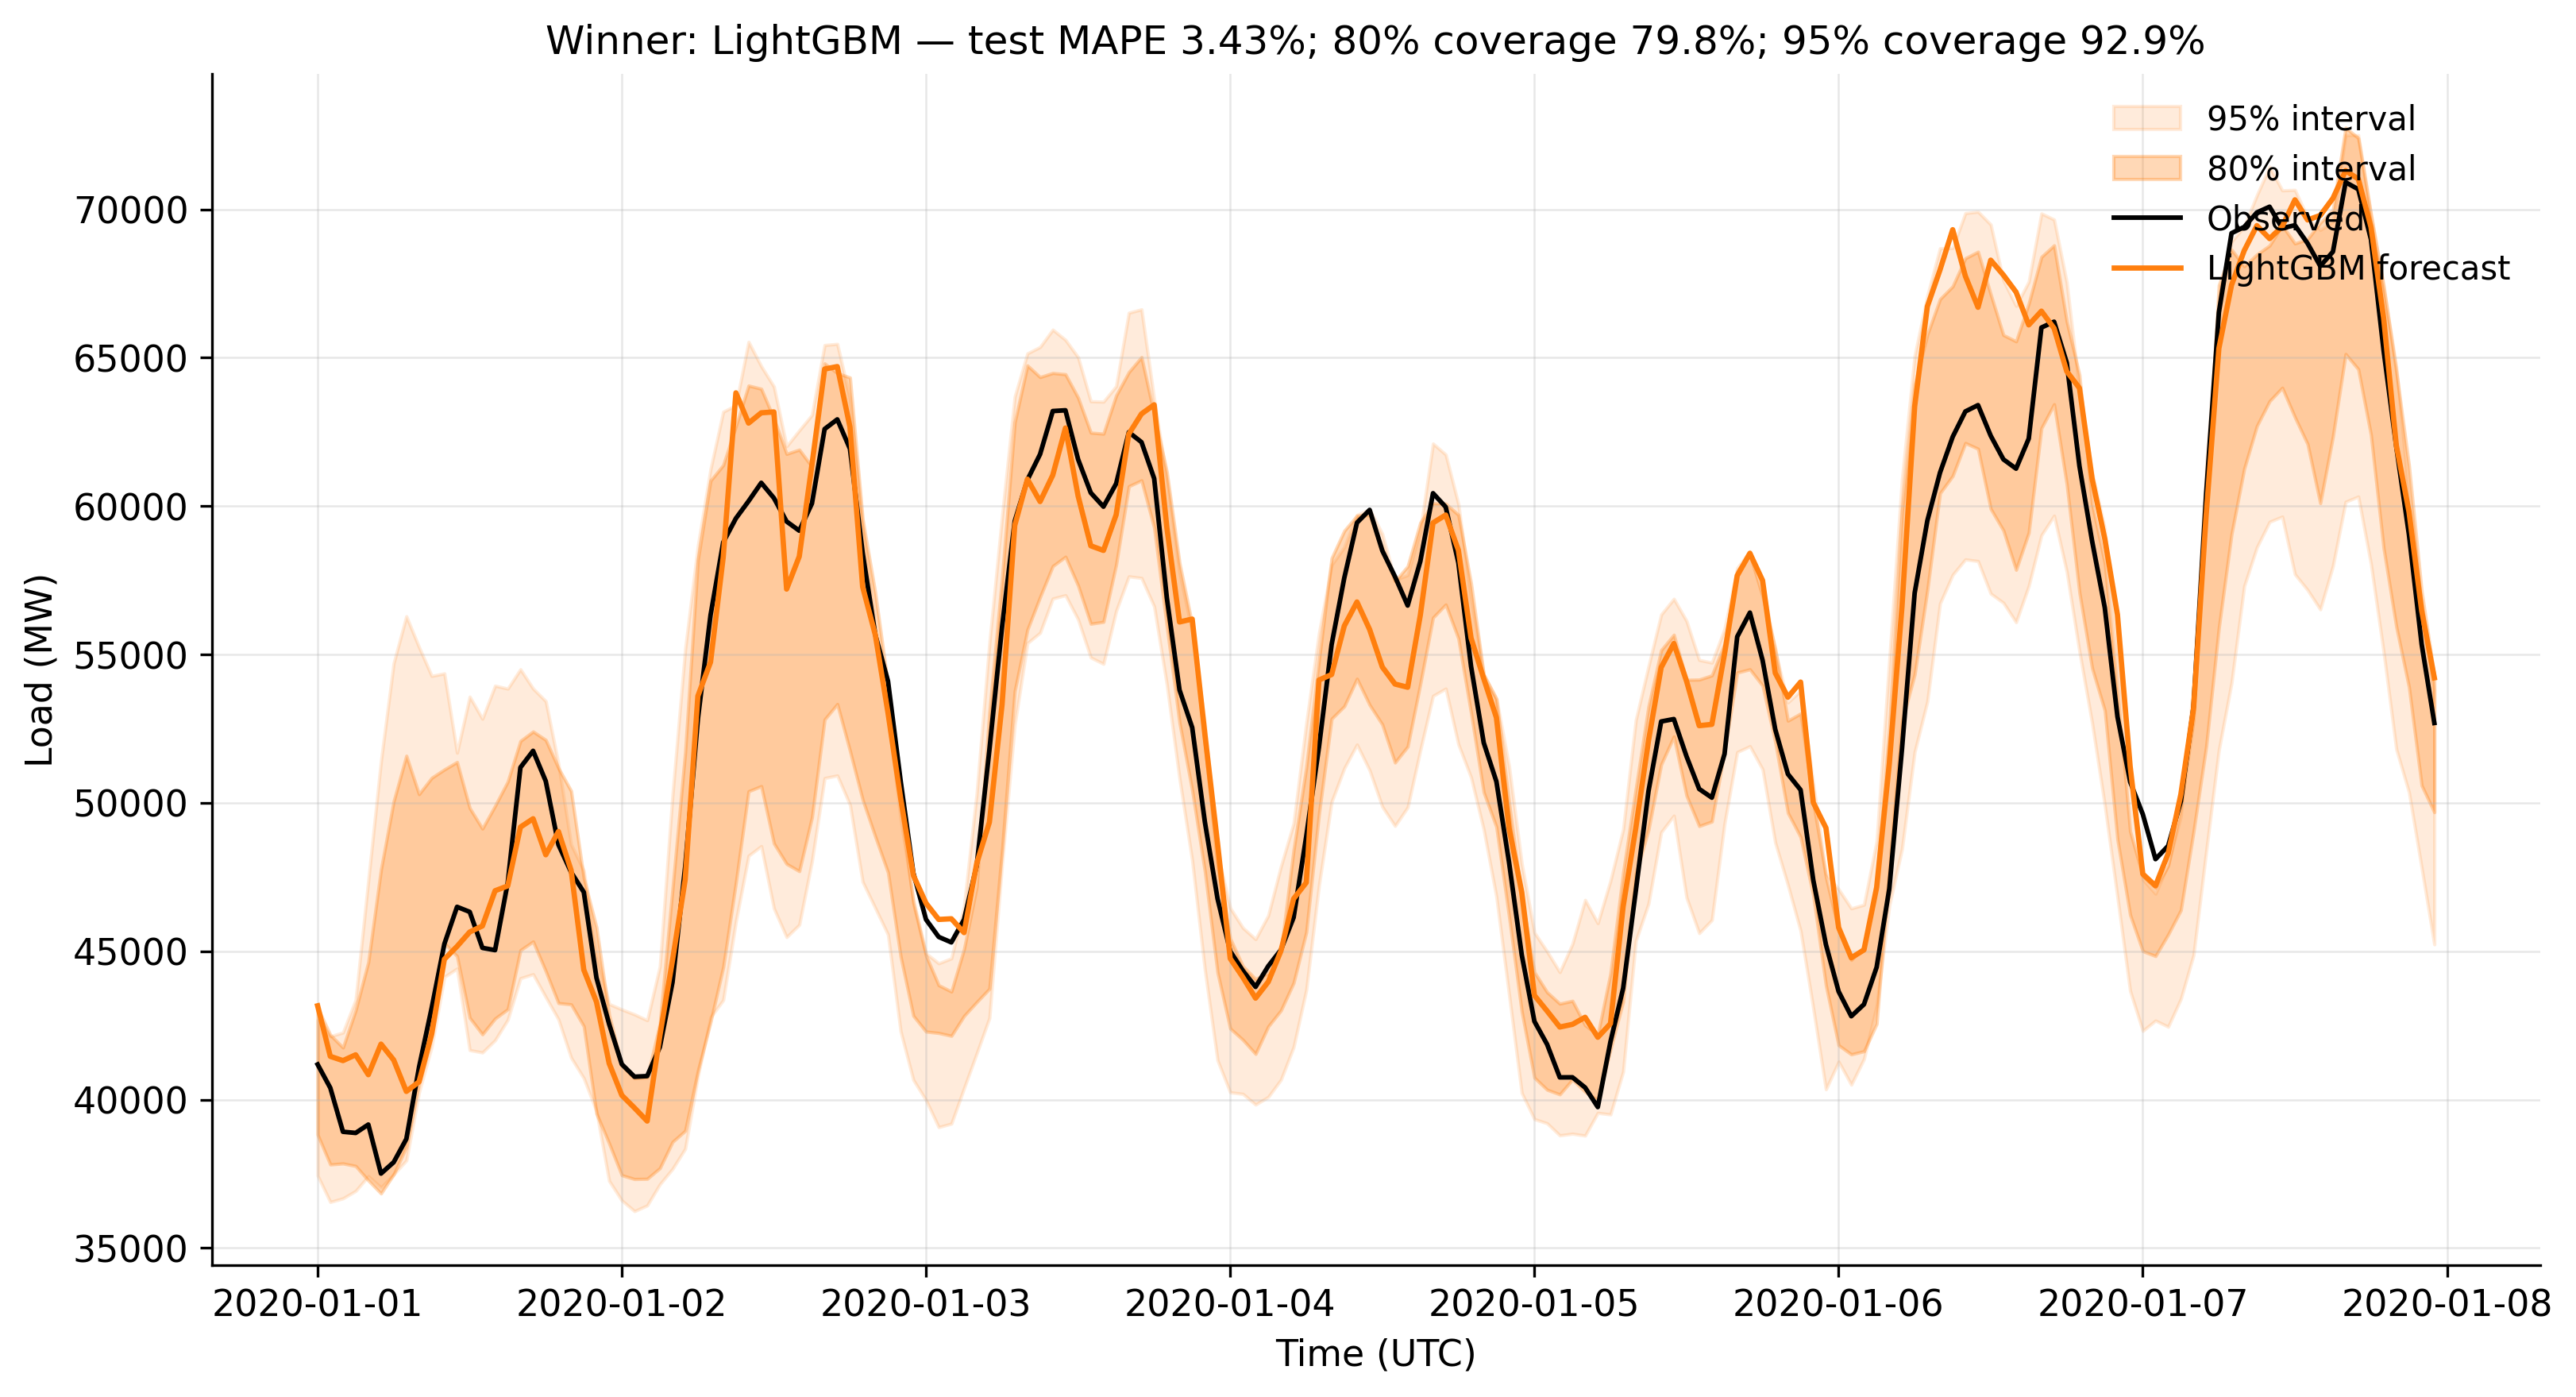
\includegraphics[height=0.52\textheight]{../runs/L3/figures/05_winner_with_intervals.png}
  \end{center}
  \begin{center}\footnotesize\color{gray!40!black}
    \textbf{LightGBM} won a six-model bake-off. \textbf{MAPE 3.43\%.}\quad
    80\% PI covered \textbf{79.8\%} \textperiodcentered{} 95\% PI covered \textbf{92.9\%} \textemdash{} essentially nominal.
  \end{center}
  \begin{center}\footnotesize\color{gray!50!black}
    L2 might have got lucky picking a decent model.\\
    L3 didn't have to be lucky \textemdash{} it searched, validated, calibrated, and documented.
  \end{center}
\end{frame}

% ===== Slide 8 — Some of what L3 produced =====
\begin{frame}{Some of what L3 actually produced}
  \begin{tcbraster}[raster columns=3, raster equal height=rows, raster row skip=2mm, raster column skip=2mm,
                    boxrule=0.4pt, colback=white, colframe=gray!30, arc=1pt,
                    halign=center, valign=center, left=2pt, right=2pt, top=2pt, bottom=2pt,
                    fontupper=\tiny]
    \tcbox[colframe=gray!30]{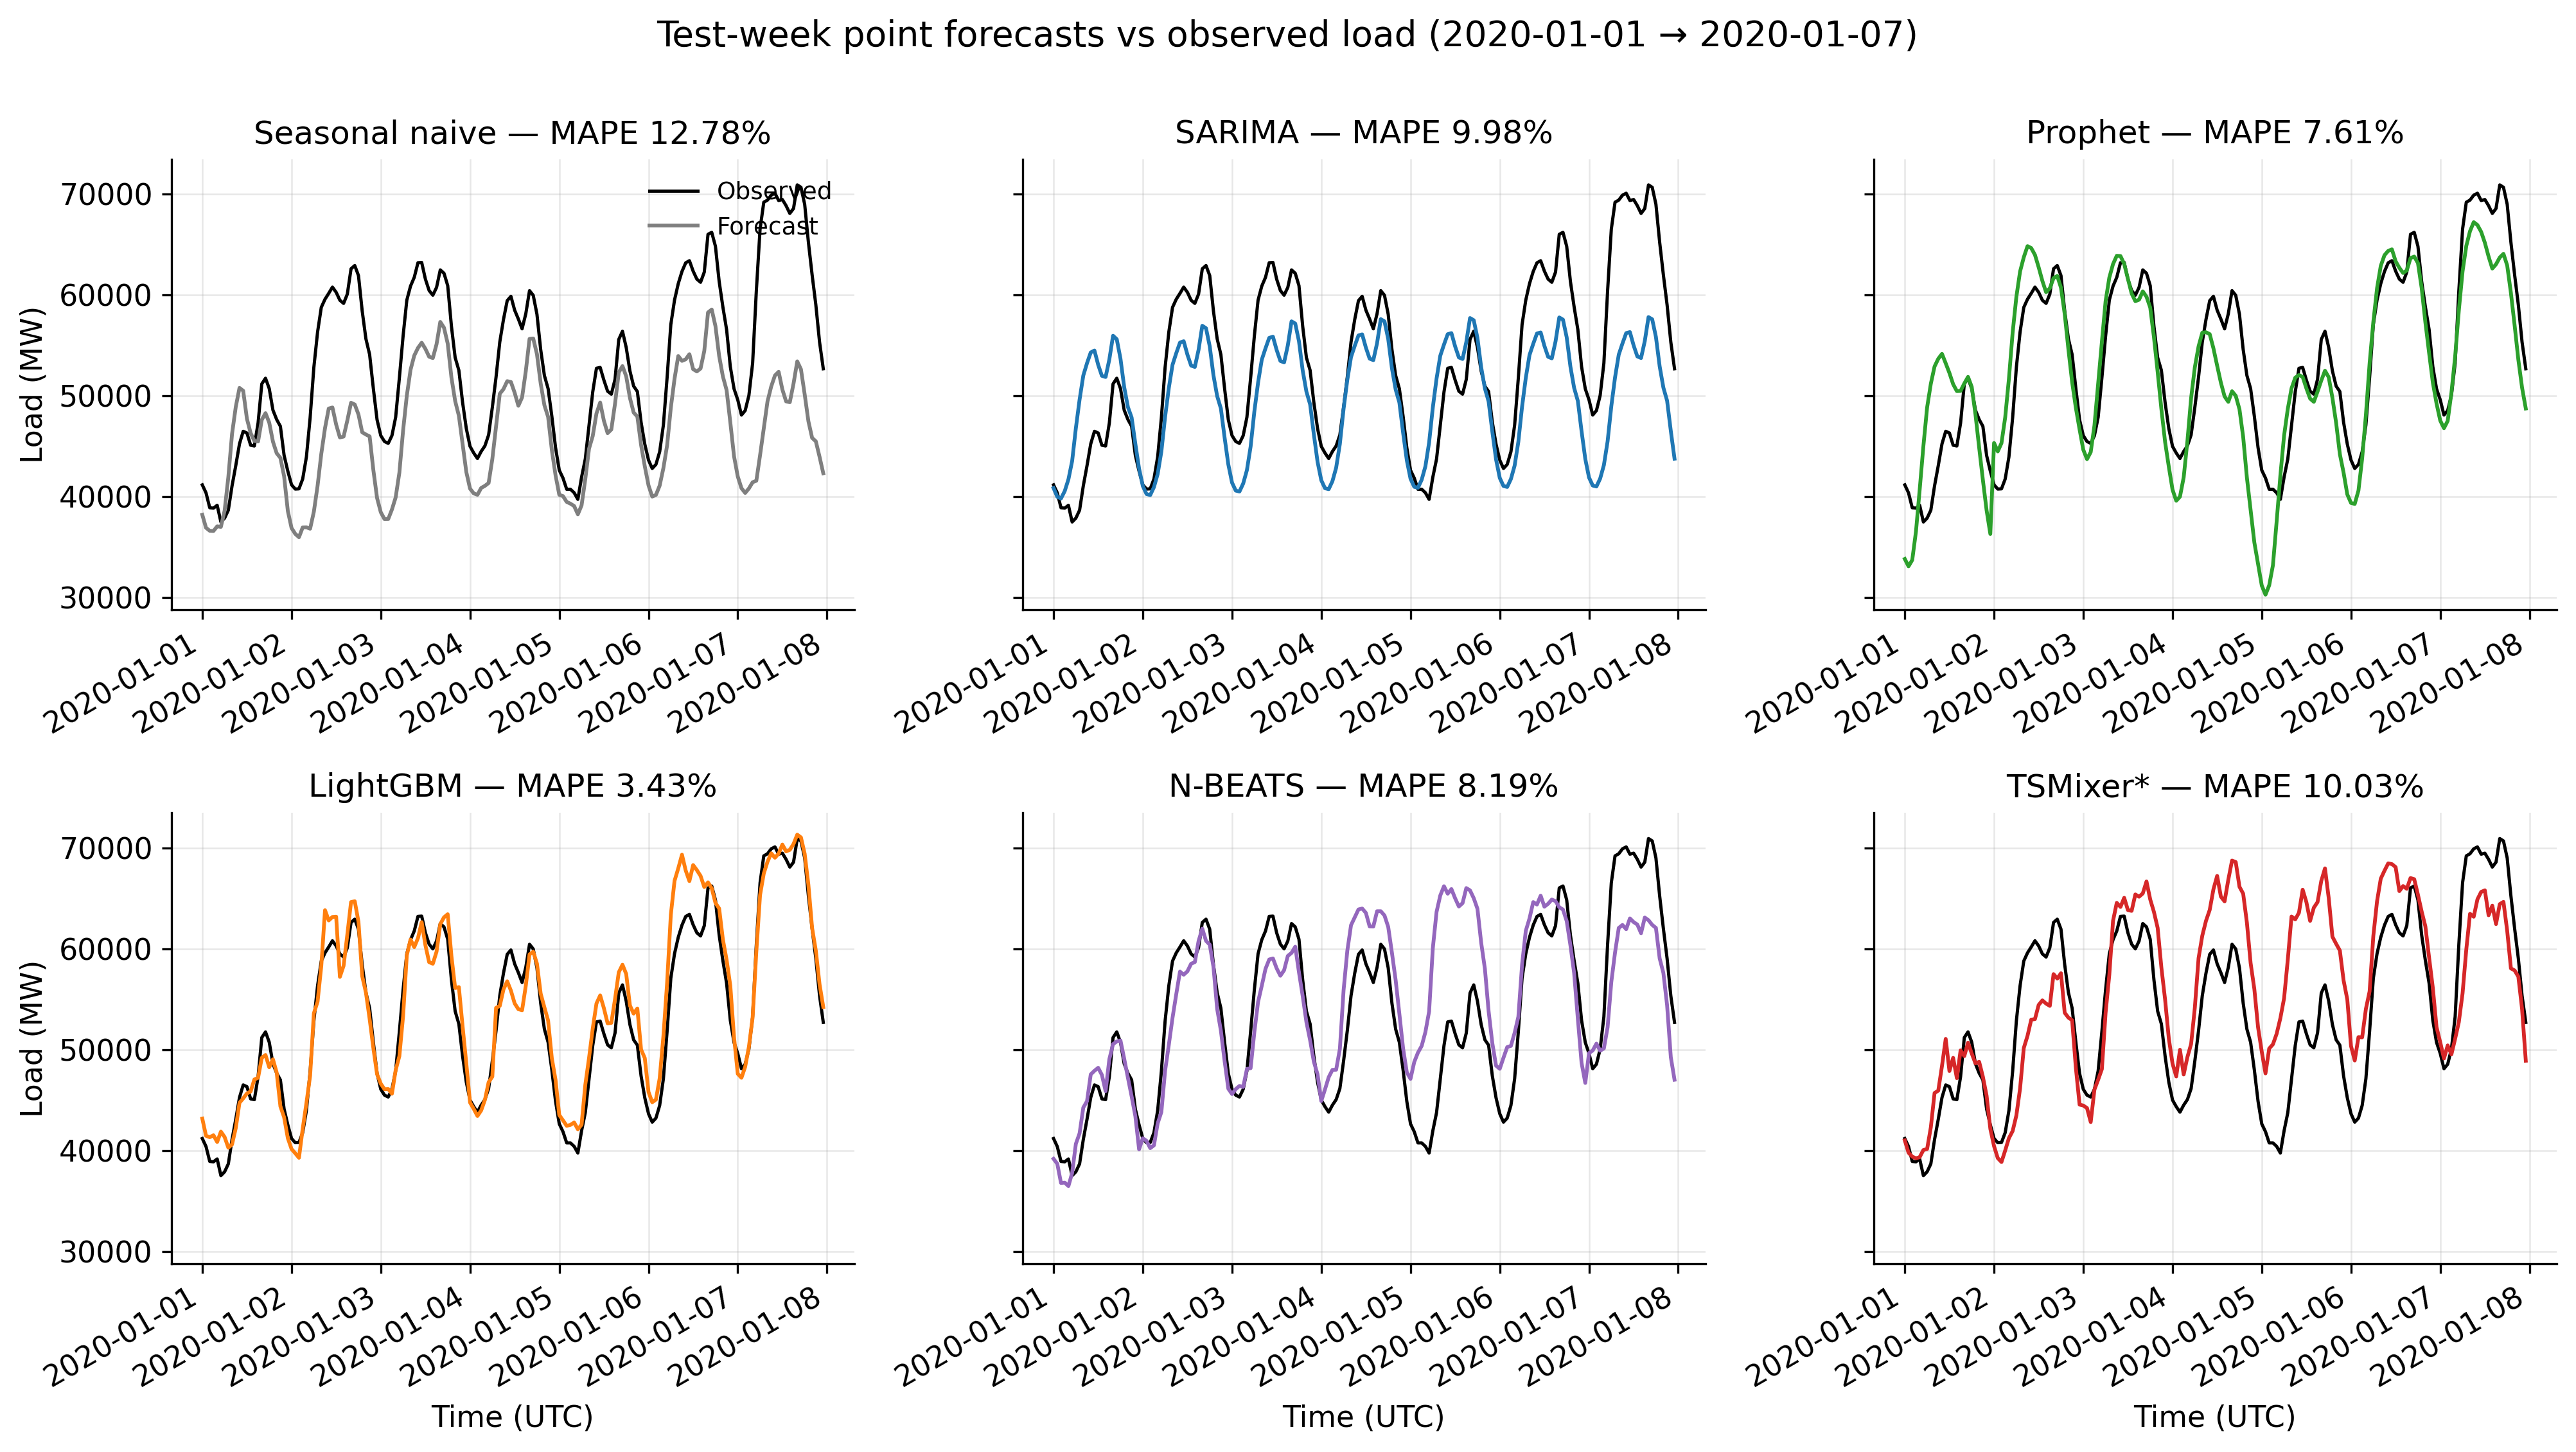
\includegraphics[width=0.97\linewidth]{../runs/L3/figures/02_forecast_comparison.png}\\Six-model comparison}
    \tcbox[colframe=gray!30]{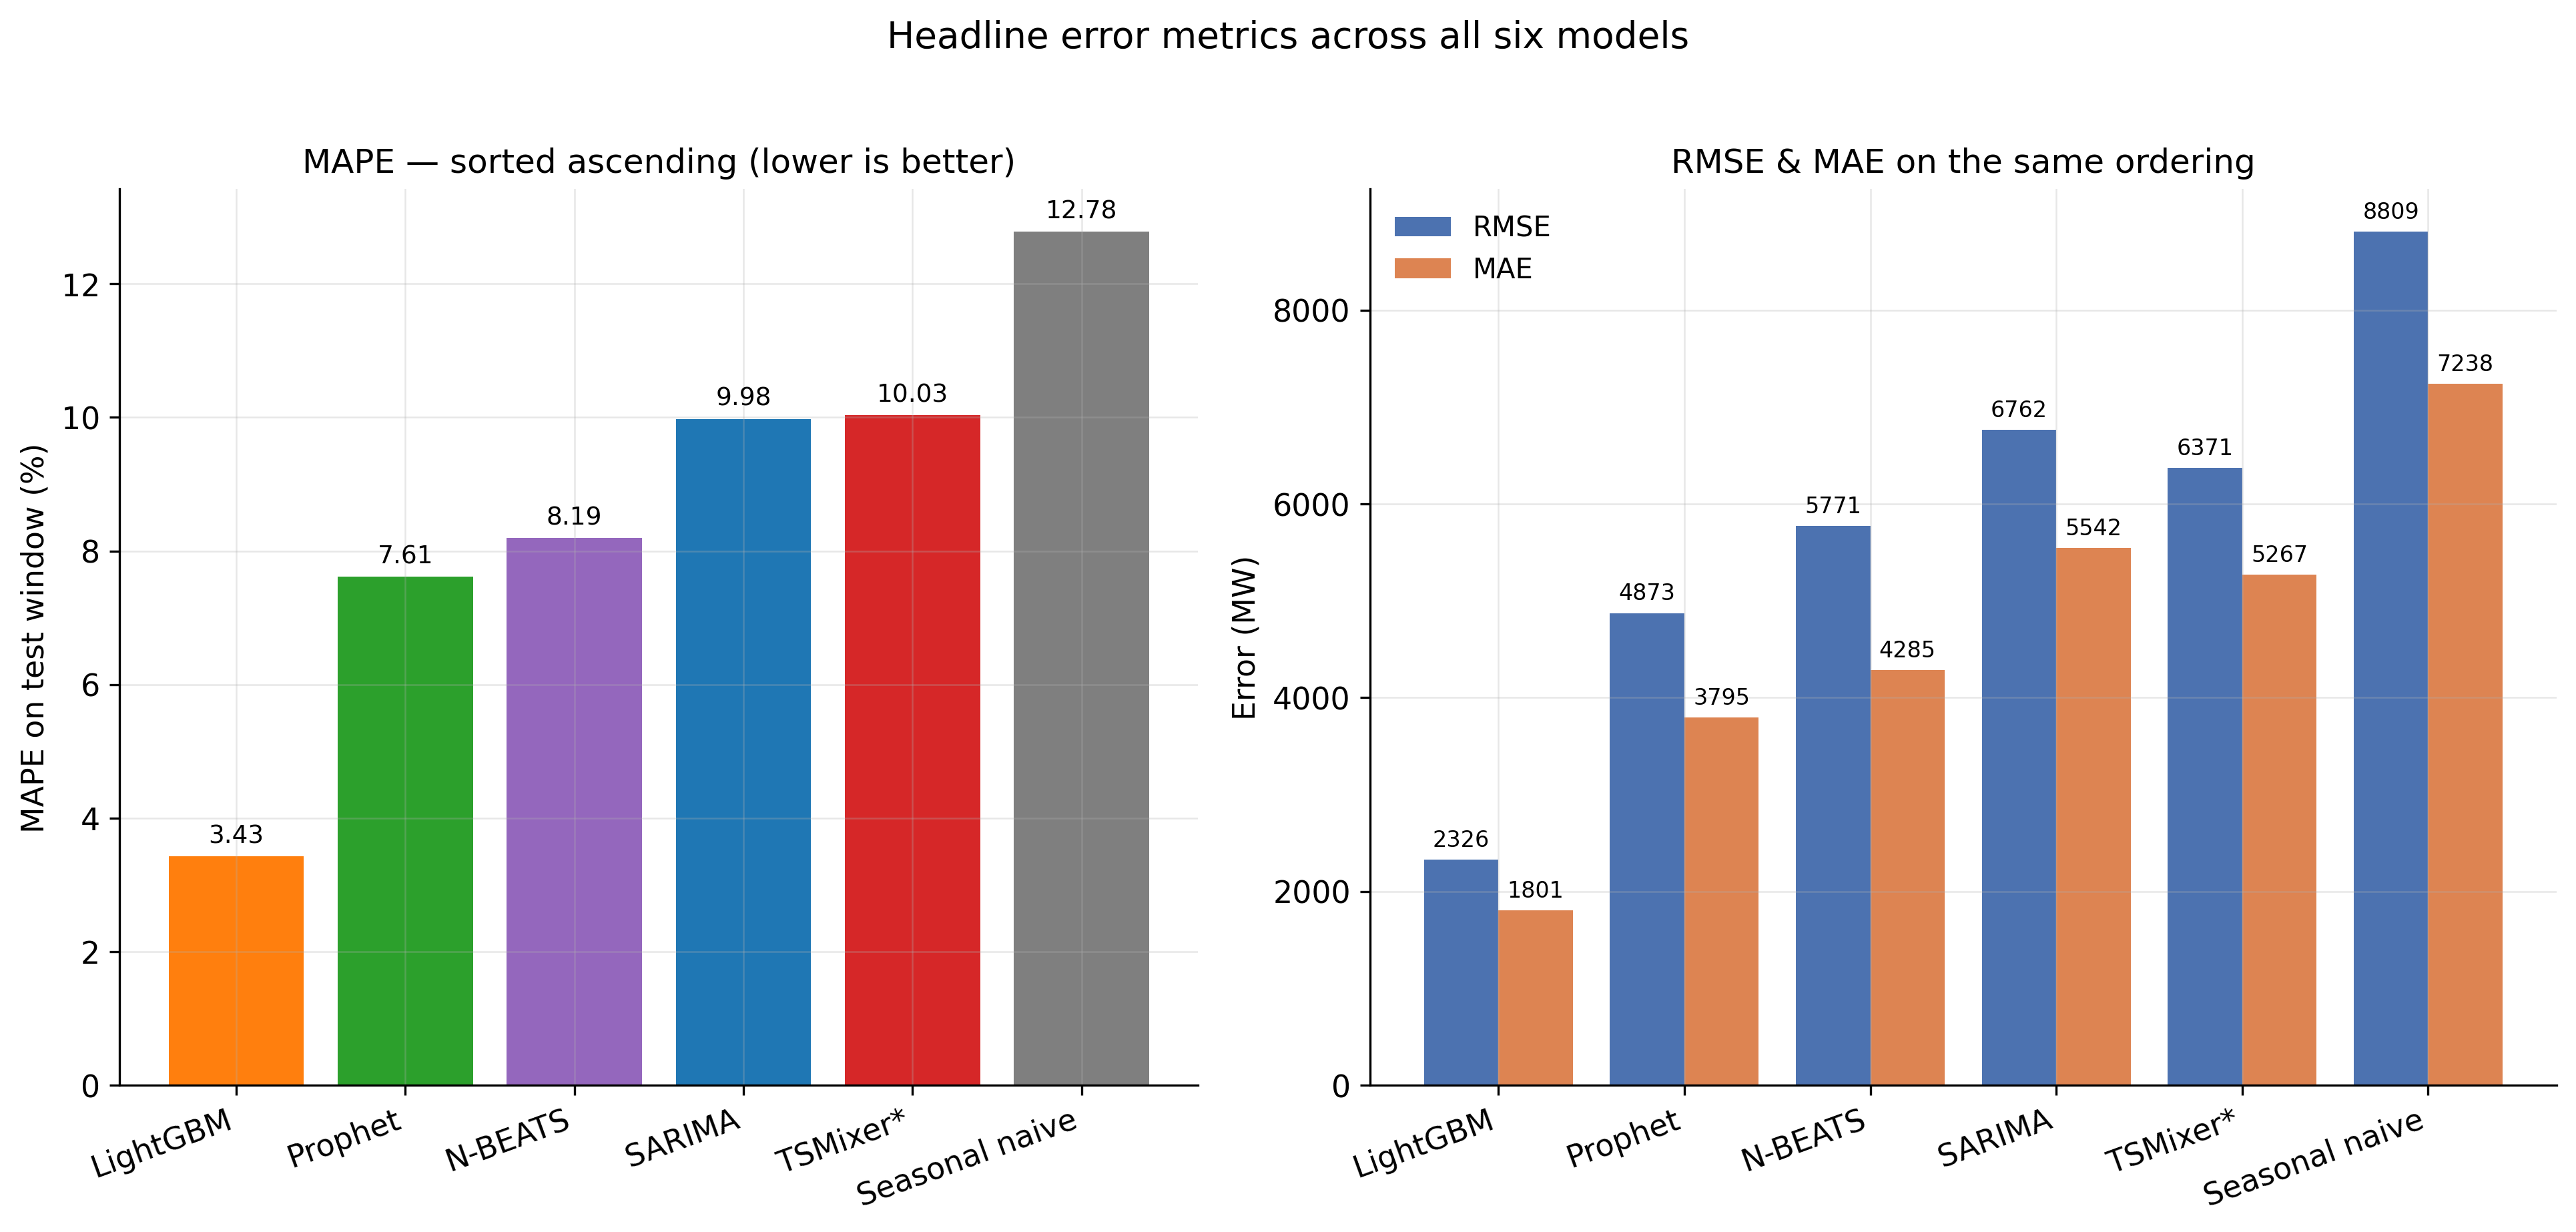
\includegraphics[width=0.97\linewidth]{../runs/L3/figures/03_metric_comparison.png}\\Scoreboard \textemdash{} MAPE, RMSE, MAE}
    \tcbox[colframe=gray!30]{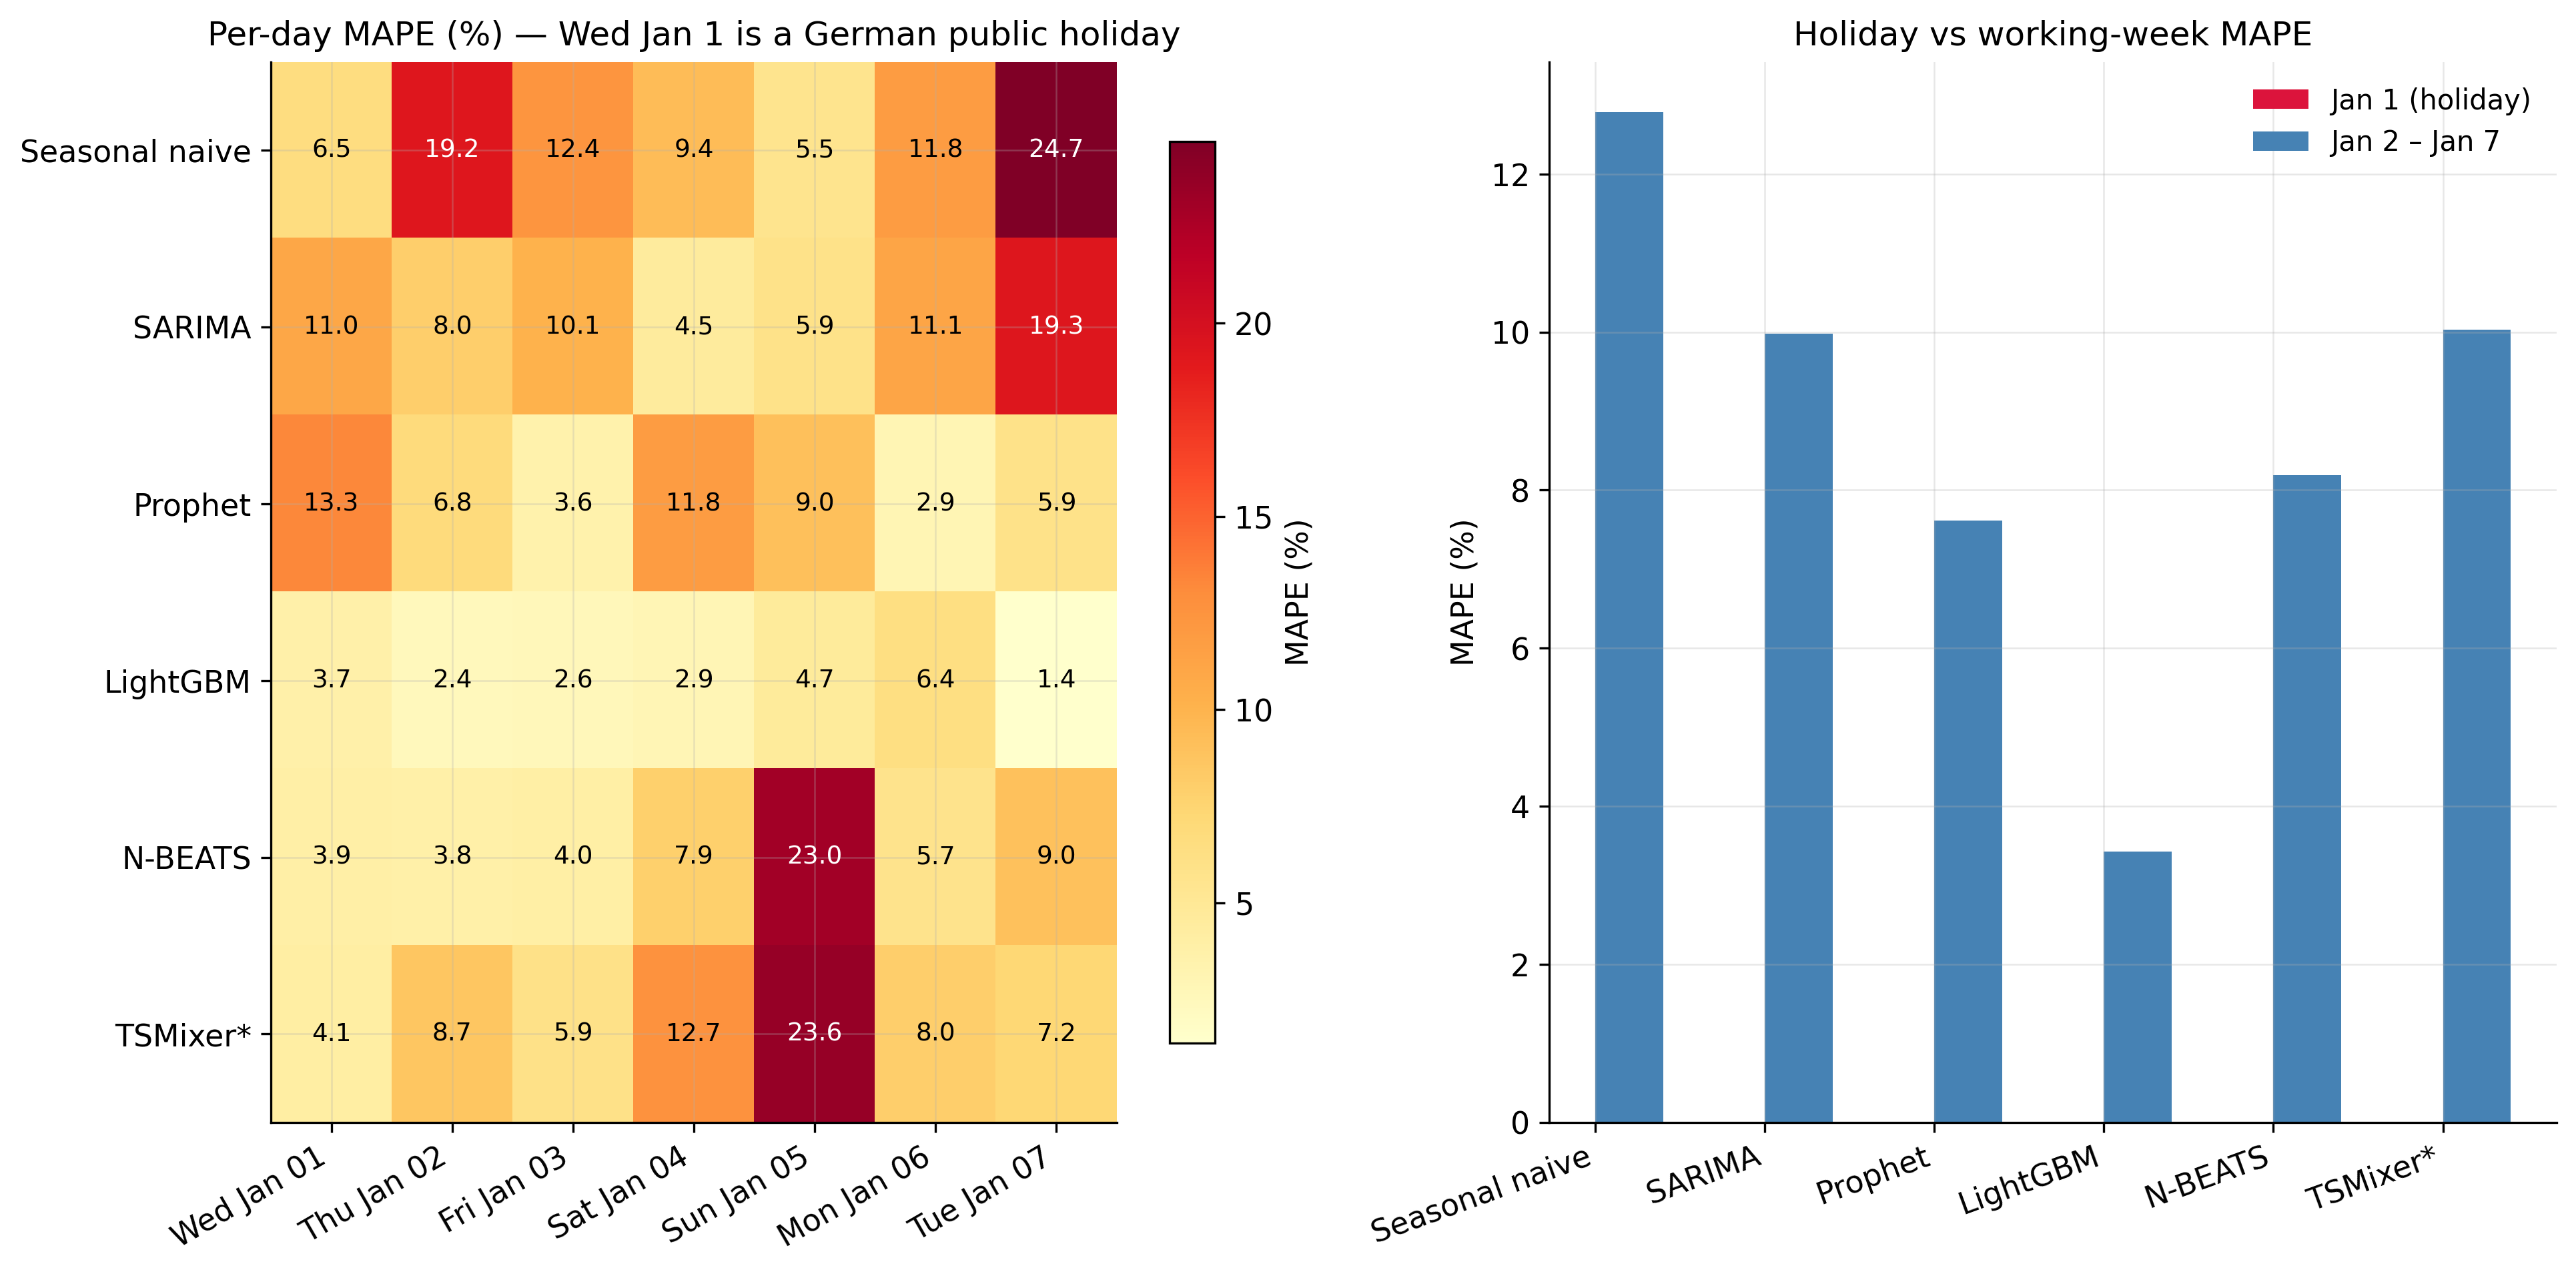
\includegraphics[width=0.97\linewidth]{../runs/L3/figures/04_per_day_mape.png}\\Per-day MAPE heatmap}
    \tcbox[colframe=gray!30]{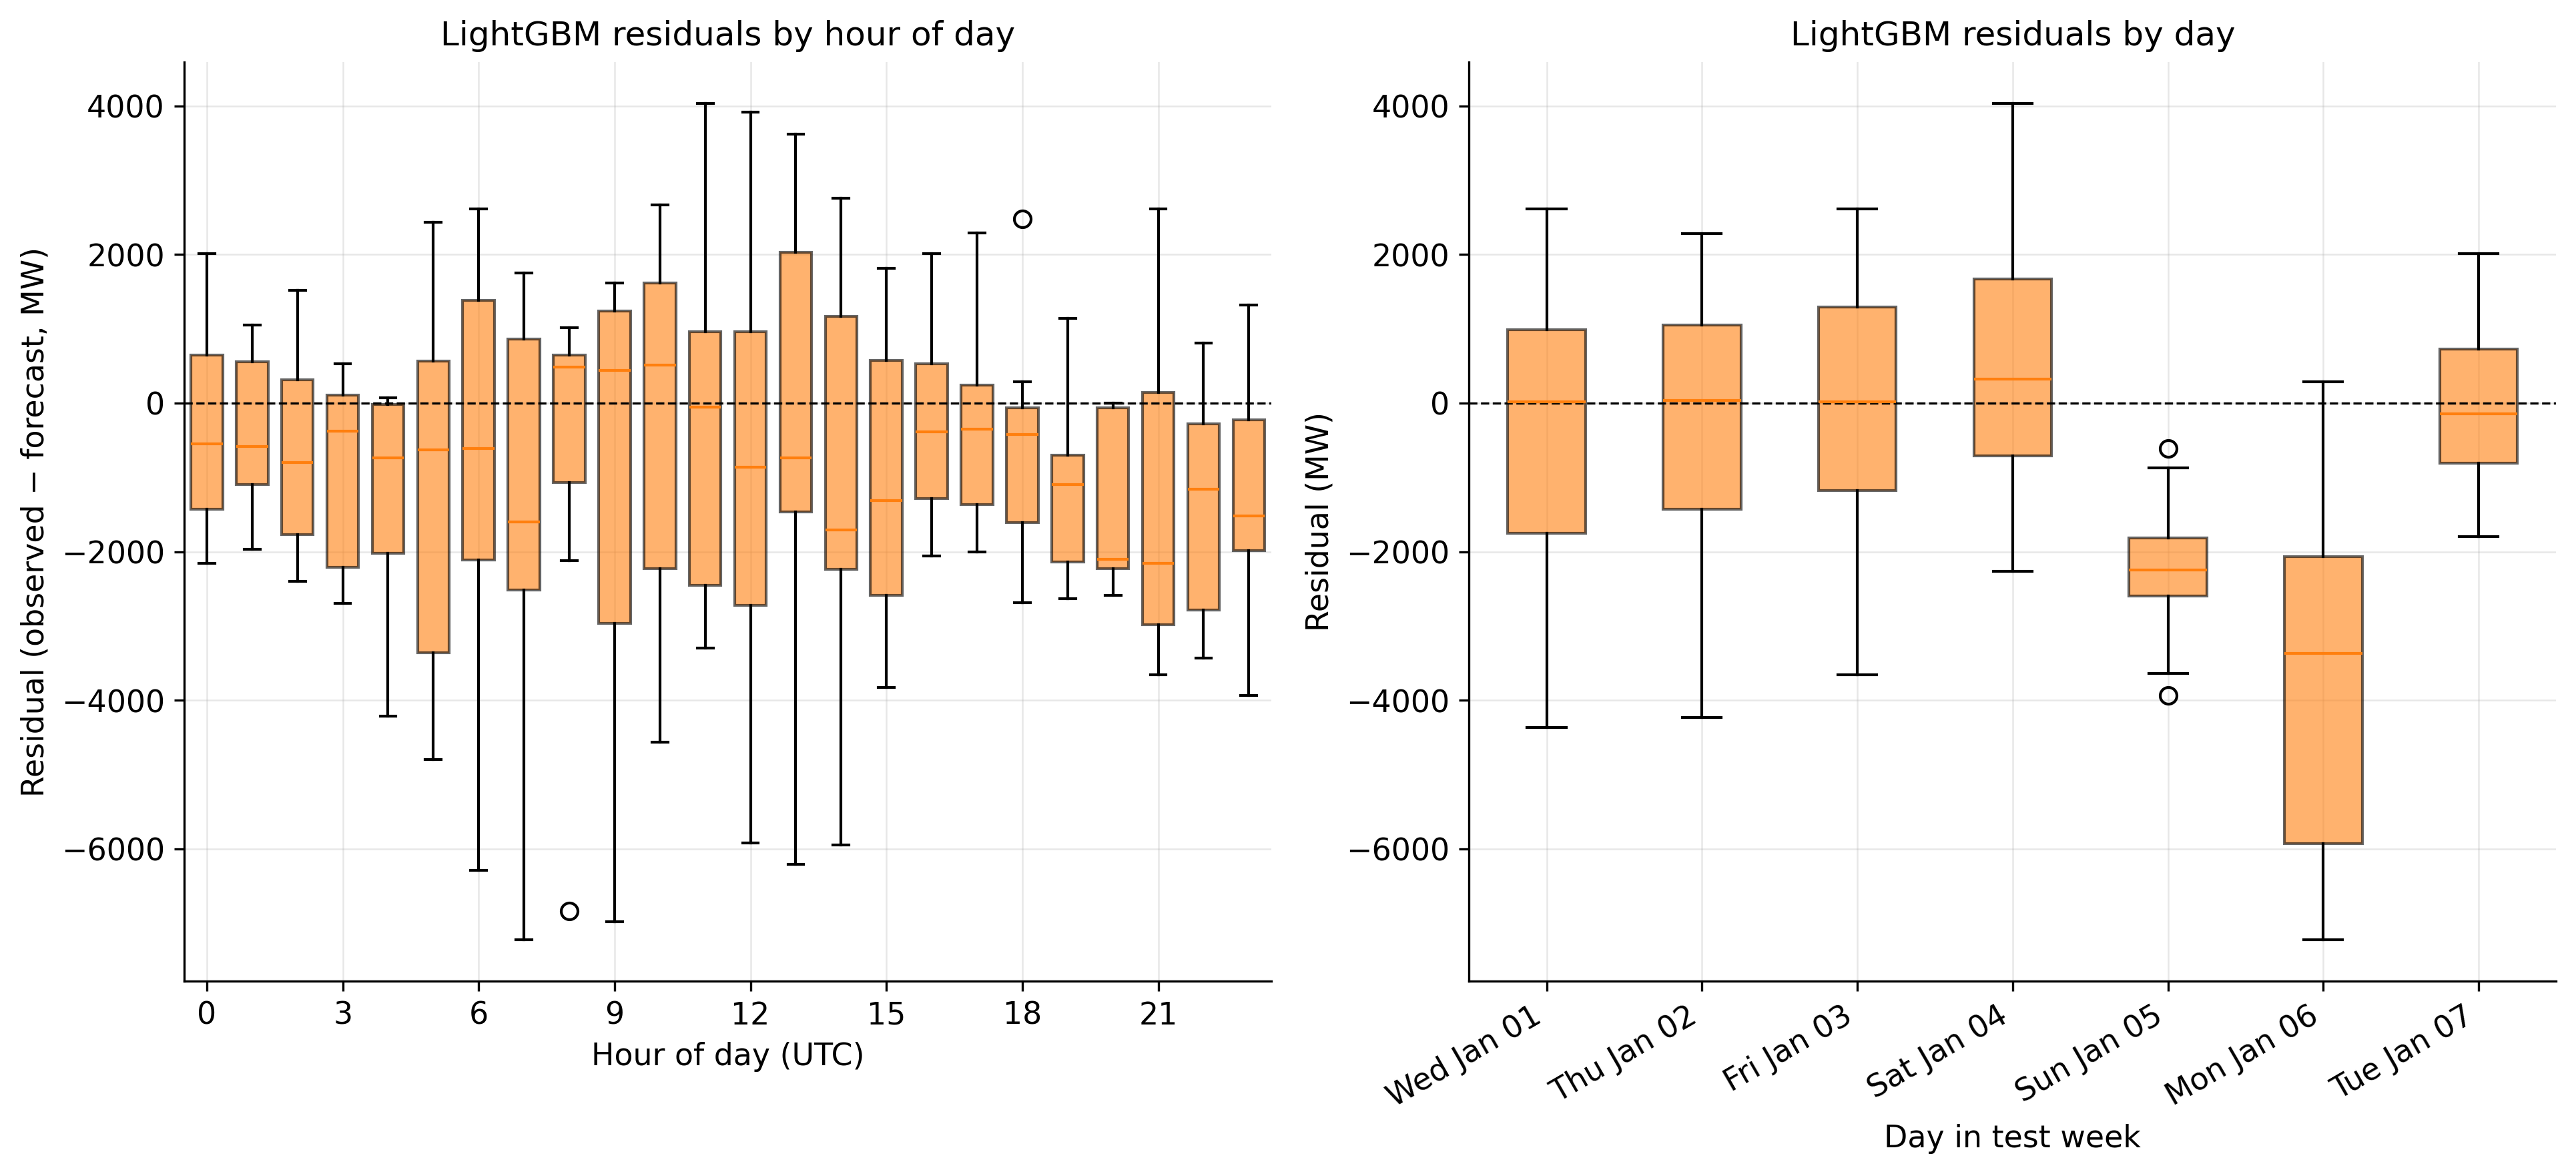
\includegraphics[width=0.97\linewidth]{../runs/L3/figures/06_residuals.png}\\Winner residuals by hour and day}
    \tcbox[colframe=gray!30]{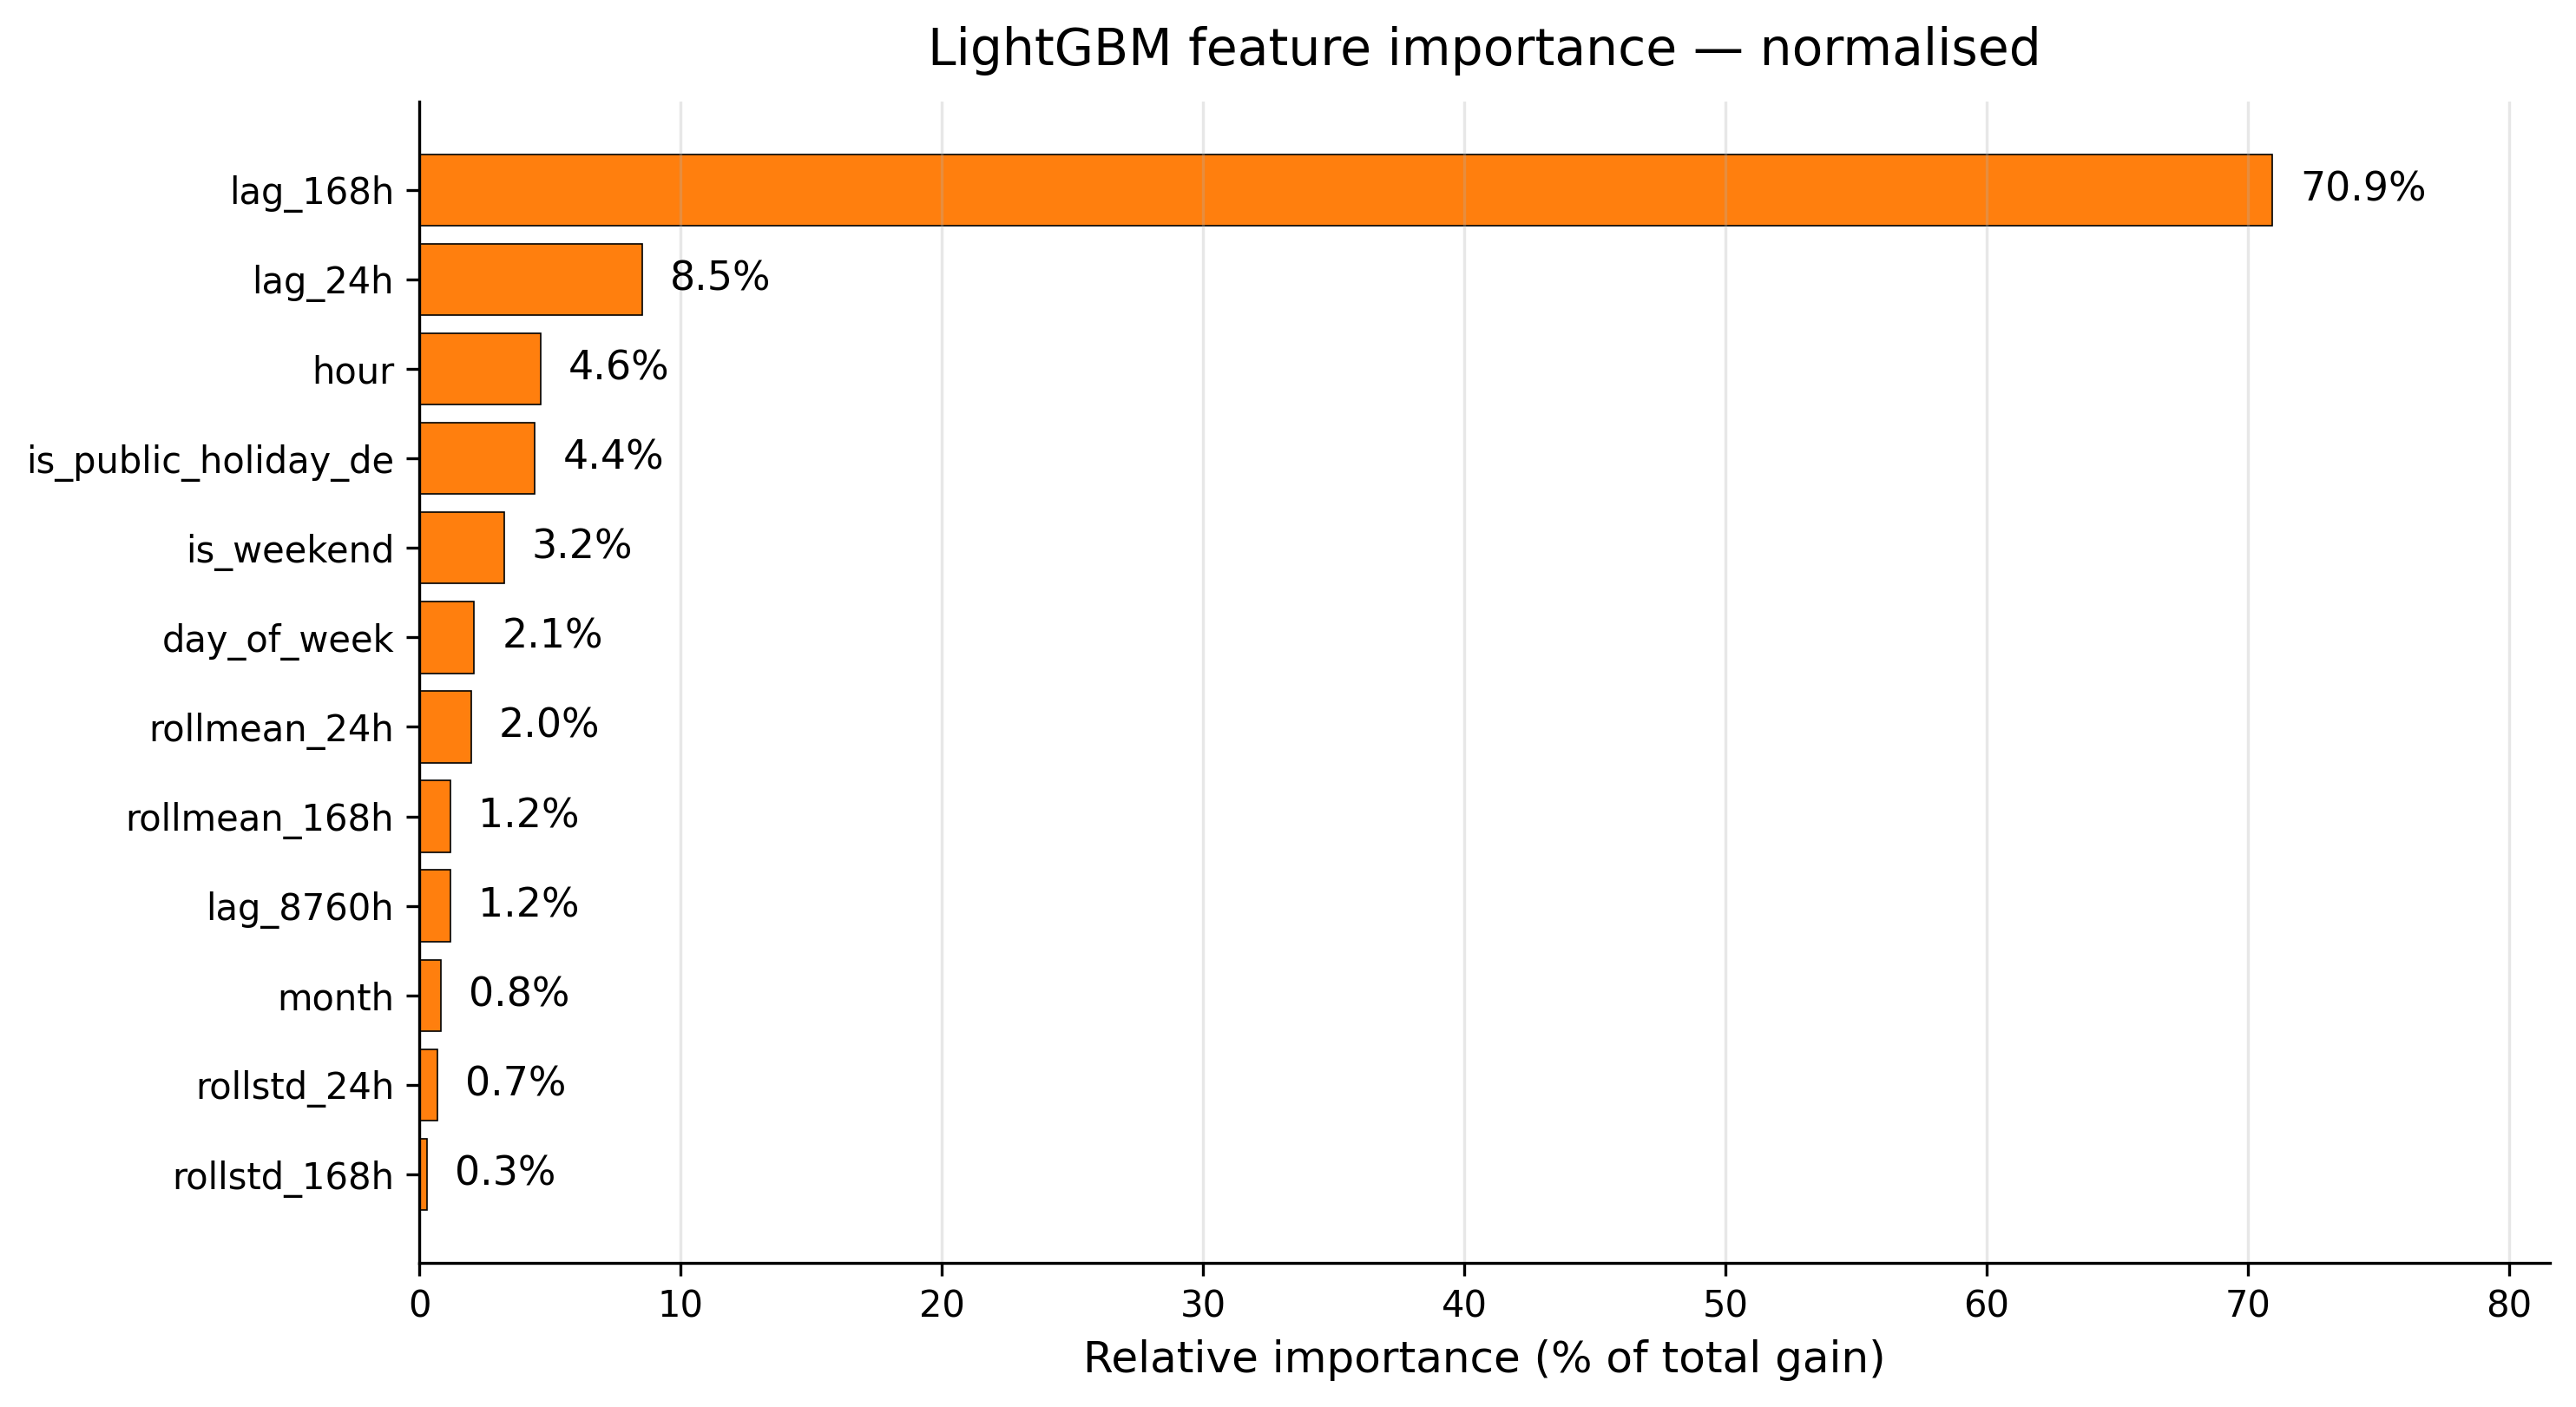
\includegraphics[width=0.97\linewidth]{assets/07_feature_importance_normalised.png}\\Feature importance (normalised)}
    \tcbox[colframe=gray!30]{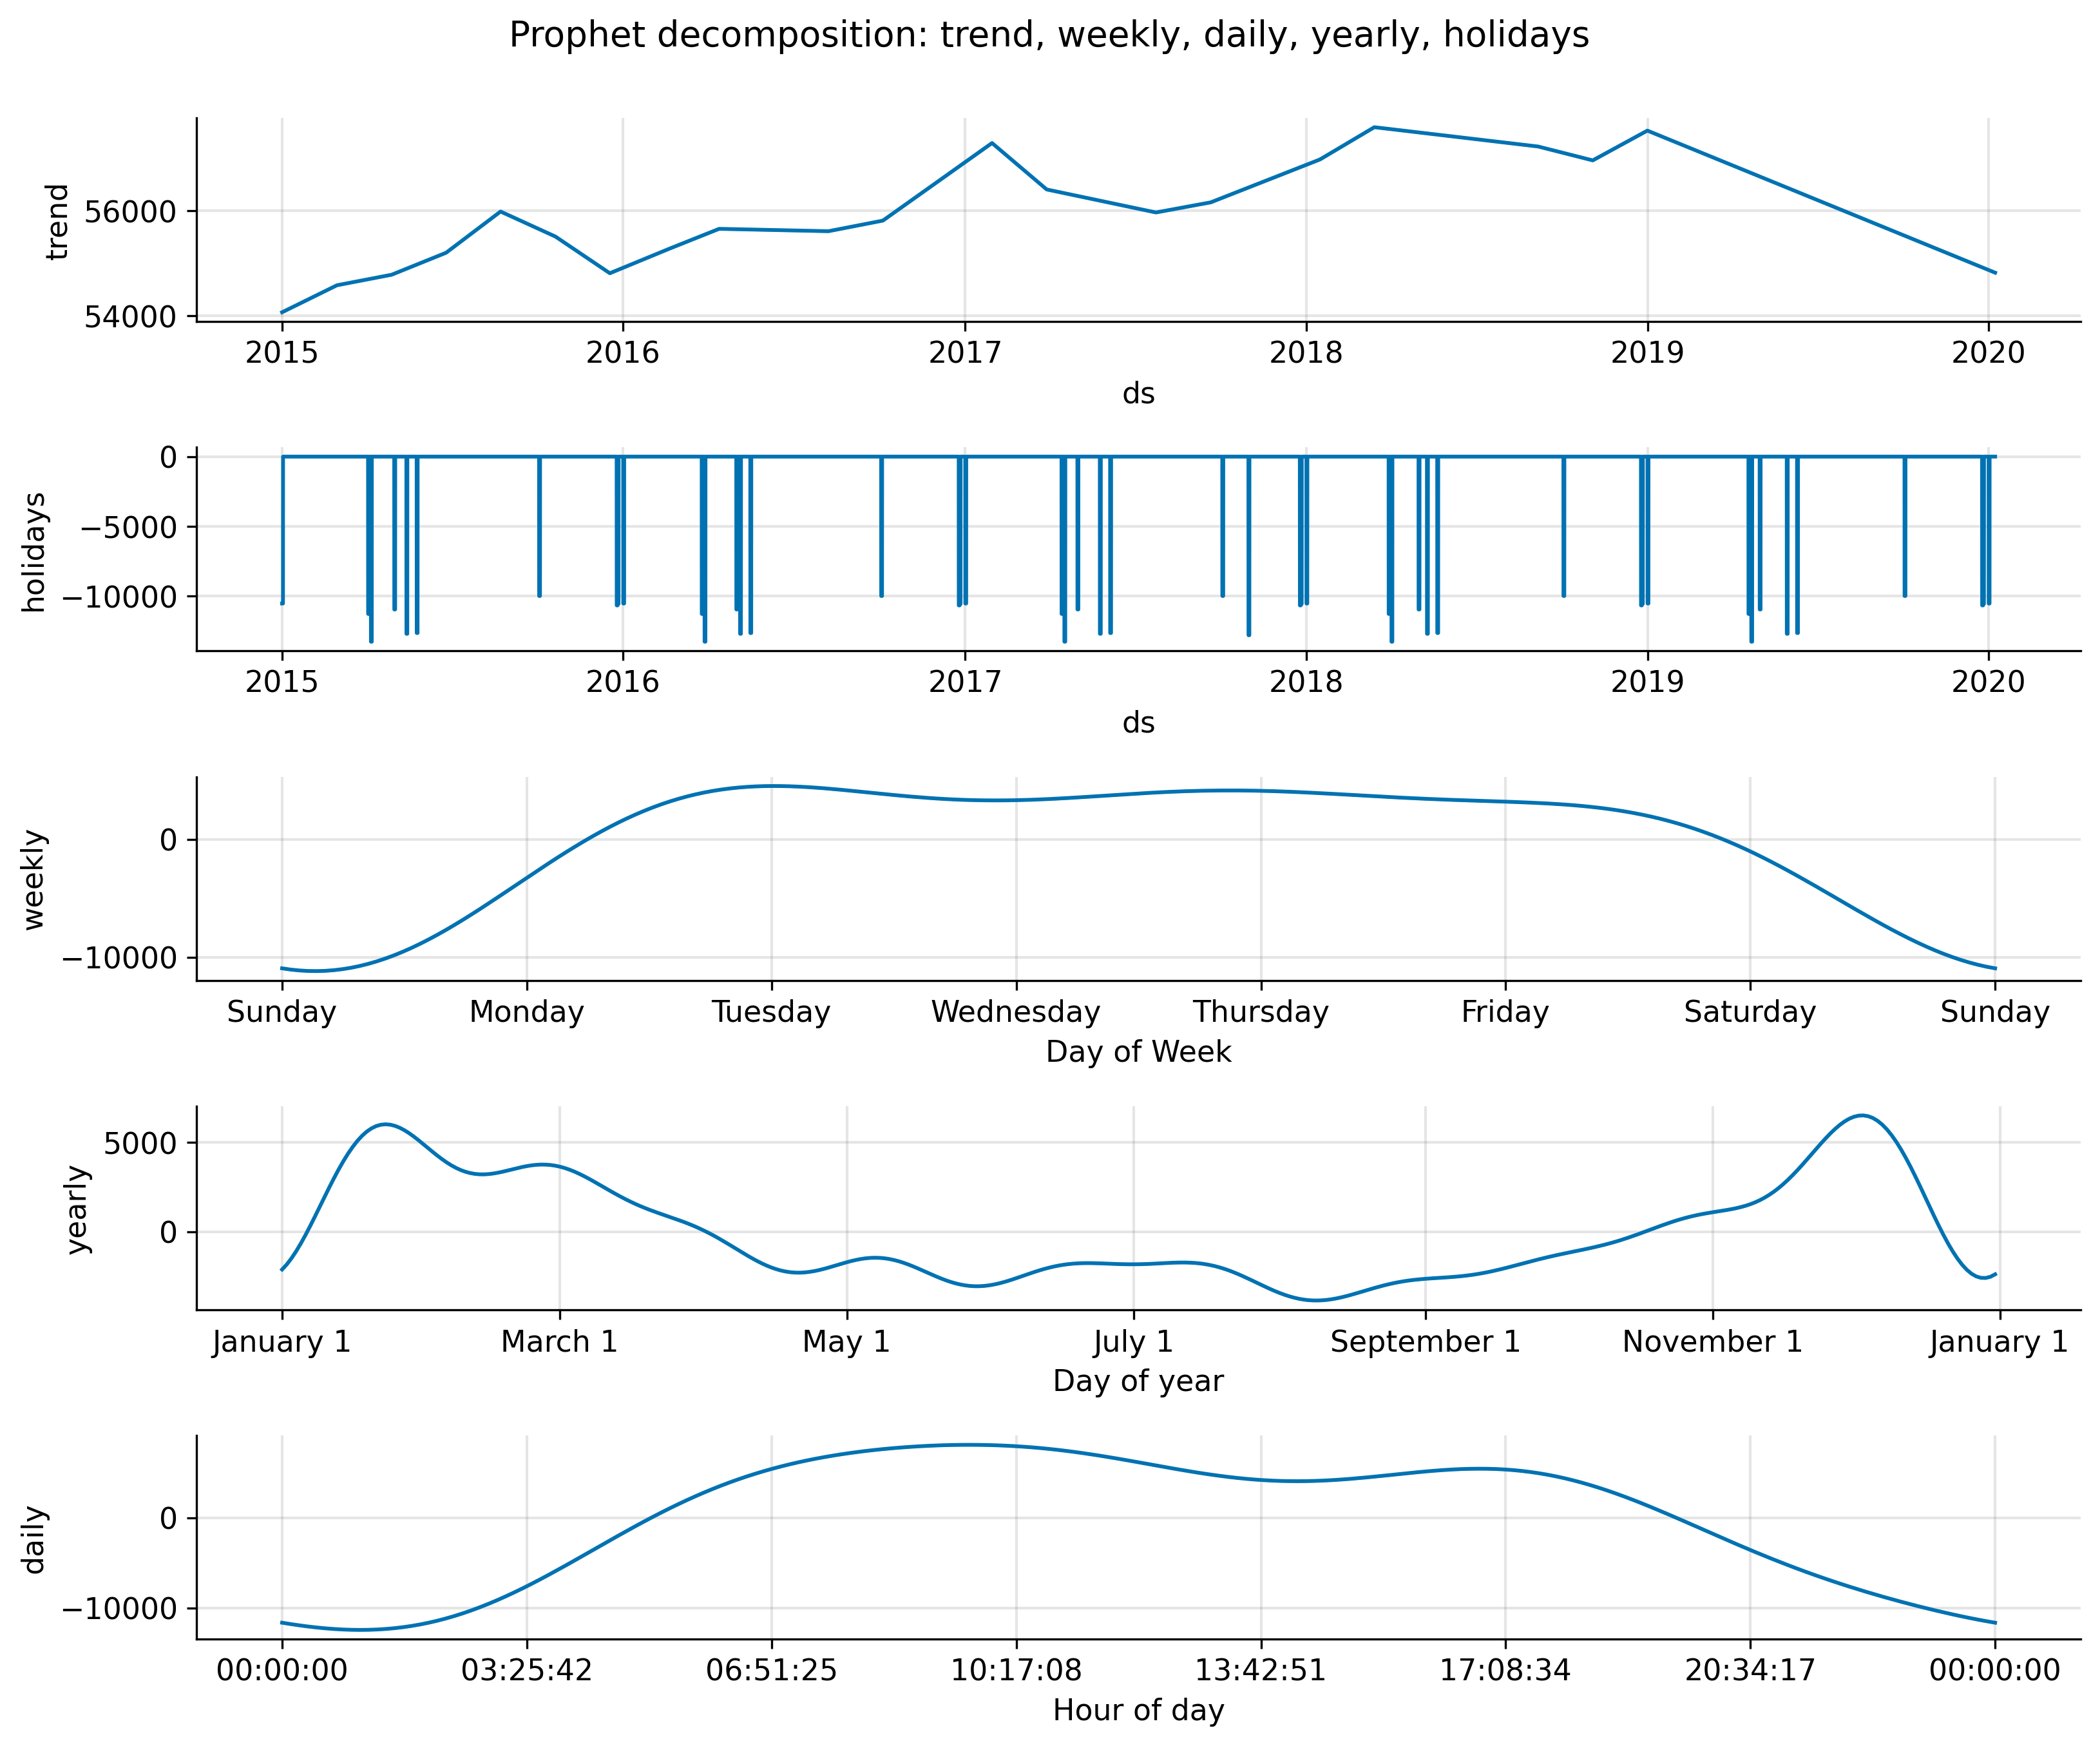
\includegraphics[width=0.97\linewidth]{../runs/L3/figures/08_decomposition.png}\\Prophet trend / seasonal decomposition}
  \end{tcbraster}
  \vspace{-4pt}
  \begin{center}\footnotesize\color{gray!40!black}
    L1 produced 1 figure. L3 produced 8.
  \end{center}
\end{frame}

% ===== Slide 9 — Tips 6, 7 + Closing thesis =====
\begin{frame}{Seven tips for working with AI (cont.)}
  \begin{columns}[t,onlytextwidth]
    \begin{column}{0.49\textwidth}
      \tipcard{TIP 6}{MCPs extend what AI can do}{%
        Plug-in tools at runtime. Context7 (docs), Hugging Face (papers), GitHub (repos).}
      \tipcard{TIP 7}{Always give AI a way to verify its work}{%
        Tests, held-out validation, calibrated intervals. Have AI generate them \emph{and} read what it wrote
        \textemdash{} AI-written tests can ``pass'' while testing the wrong thing.}
    \end{column}
    \begin{column}{0.49\textwidth}
      \begin{tcolorbox}[colback=jrcblue!8, colframe=jrcblue, boxrule=1.5pt, arc=3pt,
                        left=10pt, right=10pt, top=8pt, bottom=8pt, fontupper=\small]
        {\color{jrcblue}\textbf{\large Closing thesis}}\\[6pt]
        \textbf{AI amplifies the habits you already have.}\\[6pt]
        Let it type for you \textemdash{} not think for you.\\[6pt]
        Bring good engineering habits and AI multiplies them.\\[6pt]
        Skip tests, skip docs, skip the ``what could go wrong'' question \textemdash{} and AI amplifies \emph{that} instead.
      \end{tcolorbox}
    \end{column}
  \end{columns}
\end{frame}

\end{document}
